\documentclass{article}
\title{Assessing Toxicity in Wikipedia Comments}
\author{Jonathan Innis, Gabriel Britain}
\date{}
\usepackage{graphicx}


\begin{document}
\begin{titlepage}
	\maketitle
	\tableofcontents{}
\end{titlepage}

\begin{abstract}
	As the number of users on the internet increases, so do the number of
	obscene, hateful, or otherwise-toxic comments, and the need to moderate
	those comments. We present a text classifier model to determine whether
	a model is toxic or not, and if toxic, in what way. The topic was
	originally presented as a \$35,000 competition on Kaggle, and uses data
	as provided by Wikipedia talk page edits
	\cite{Wulczyn:2017:EMP:3038912.3052591}. A number of models were
	developed through trial-and-error to classify comments. Specifically
	developed models were Naive Bayes, support-vector machines, random
	forest classifiers, and a GloVe embedding-based recurrent neural
	network.
\end{abstract}

\section{Dataset Source \textit{Gabriel Britain}}{
  The dataset used can be found on Kaggle under the "Toxic Comment
  Classification Challenge." Another participant in the challenge
  performed data augmentation by running the original training dataset
  repeatedly through Google Translate, and then including the results as
  training data. This augmented data, however, could lead to significant
  overfitting, as discussed later.
 }

\section{Frameworks \textit{Gabriel Britain}}{
  For data analyis and graphing, pandas\cite{mckinney-proc-scipy-2010}
  and matplotlib\cite{Hunter:2007} were used. For the process of actual
  machine learning model building, rather than spending a significant amount
  of time implementing different models from scratch, and to focus efforts on
  feature engineering, architecture design, and hyperparameter optimization,
  scikit-learn\cite{sklearn_api} and Keras\cite{chollet2015keras} were used.
  \subsection{Pandas}{
	  Pandas is an open-source library that provides high-performance and
	  easy-to-use data structures for processing and analyzing CSV data.
	  Pandas was used for data inspection, analyzing class imbalances, and
	  reporting results of developed algorithms.
  }
  \subsection{Matplotlib}{
	  Matplotlib is a Python 2D plotting library which produces high-quality
	  figures easily. Matplotlib was used occasionally for plotting the
	  distribution of words, characters, phrases, and class imbalances.
  }
  \subsection{Scikit-Learn}{
	  Scikit-Learn (sklearn) is a simple and efficient machine learning framework
	  that implements many machine learning algorithms and packages them in
	  simple, easy-to-use Python classes. Hyperparameters for these machine
	  learning algorithms are available as Python class attributes, which makes
	  hyperparameter tuning a very simple task. In addition, sklearn implements
	  many functions that simplify the model-building workflow, such as
	  cross-validation, training-validation splits, tokenization, and metric
	  reporting, and model evaluation.
  }
  \subsection{Keras}{
	  Keras is a high-level neural networks API, written in Python and capable of
	  interfacing with TensorFlow\cite{tensorflow2015-whitepaper}. Keras was used
	  to develop a recurrent neural network model that used pre-trained GloVe word
	  embeddings\cite{pennington2014glove}, to determine if pre-trained word
	  embeddings could provide stronger and more robust models than
	  statistics-based models.
  }
 }

\section{Evaluation Metrics \textit{Jonathan Innis}}{
  The task of identifying toxic comments can be modeled as a multilabel
  classification problem. As a result, we set out to find evaluation metrics
  that were appropriate for the task. Initially, Hamming loss
  and Jaccard similarity were used as our evaluation metrics, but were found to
  be too forgiving. Thus, we settled on using F1 as our evaluation metric
  for each class. To evaluate the overall success of the
  model, we used two aggregate metrics: weighted F1 (which is the weighted
  average of F1 scores for each class), and macro F1.
  \paragraph{}As we continued to improve and evaluate our models, we became
  curious as to the performance of our models as compared to those entered in
  the original competition. We found that the original Kaggle competition was
  actually using Area under the Receiver Operating Curve (AUROC) as their
  evaluation metric for submission quality. We didn't use this metric for
  evaluating our model, but rather to compare the performance of our model with
  other submitted models.
 }
\section{Process}{
  \subsection{Data Analysis \textit{Jonathan Innis, Gabriel Britain}}{
	  Analysis began upon downloading the training dataset. The overall class
	  distribution can be seen in Figure \ref{fig:class-dist} on page
	  \pageref{fig:class-dist}.
	  \begin{figure}[h]
		  \centering
		  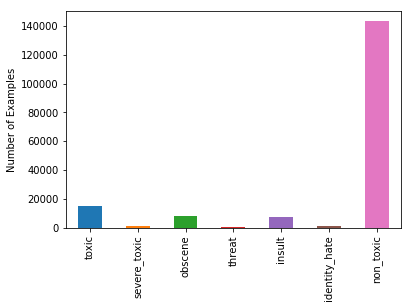
\includegraphics[width=\textwidth]{class-distribution.png}
		  \caption{Class Distribution}
		  \label{fig:class-dist}
	  \end{figure}
	  The "non-toxic" label was artificially added to indicate the number of
	  examples that are labeled as not belonging to any of the toxicity classes.
	  Clearly, the number of "non-toxic" examples dominates the number of toxic
	  examples belonging to any category. Within the toxic labels, however, there
	  is \textit{also} a class imbalance, as can be seen in Figure
	  \ref{fig:toxic-dist} on page \pageref{fig:toxic-dist}.

	  \begin{figure}[h]
		  \centering
		  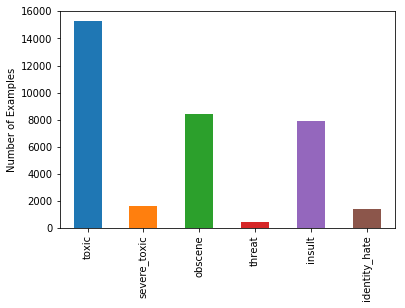
\includegraphics[width=\textwidth]{toxic-distribution.png}
		  \caption{Toxic Class Distribution}
		  \label{fig:toxic-dist}
	  \end{figure}
  }
  The "severe\_toxic", "threat", and "identity\_hate" classes are significantly
  under-represented in the toxic classes. Further data analysis can be found in
  the "Data Introspection" file under the \texttt{src} folder.

  \subsection{Establishing a Baseline \textit{Gabriel Britain}}{
	  In order to evaluate the models developed and verify that they were having
	  an actual impact on classification quality, a baseline was created using the
	  distribution of toxicity classes found. The result of the baseline on the
	  testing dataset can be found in Figure \ref{table:rand-base} on page
	  \pageref{table:rand-base}.

	  \begin{table}[h!]
		  \centering
		  \begin{tabular}{|c|| c c c c|}
			  \hline
			                                     & Precision              & Recall                 & F1-Score               & Support                 \\ [0.5ex]
			  \hline\hline
			  Toxic                              & 0.10                   & 0.06                   & 0.16                   & 5038                    \\
			  Severely Toxic                     & 0.01                   & 0.06                   & 0.02                   & 500                     \\
			  Obscene                            & 0.05                   & 0.23                   & 0.08                   & 2810                    \\
			  Threat                             & 0.00                   & 0.02                   & 0.08                   & 152                     \\
			  Insult                             & 0.05                   & 0.23                   & 0.01                   & 2591                    \\
			  Identity Hate                      & 0.01                   & 0.04                   & 0.01                   & 449                     \\
			  \hline\hline
			  Micro Average                      & 0.07                   & 0.30                   & 0.11                   & 11540                   \\
			  Macro Average                      & 0.04                   & 0.17                   & 0.06                   & 11540                   \\
			  \textit{\textbf{Weighted Average}} & \textit{\textbf{0.07}} & \textit{\textbf{0.30}} & \textit{\textbf{0.11}} & \textit{\textbf{11540}} \\

			  \hline
		  \end{tabular}
		  \caption{Random Baseline Results}
		  \label{table:rand-base}
	  \end{table}
  }
 }

\section{Model Development}{
  \subsection{Feature Engineering \textit{Gabriel Britain}}{
	  Initially, the only feature used in training each model was the tokenized
	  document corpus as a bag-of-words (BOW), represented through TF-IDF vectors.
	  However, we soon realized that there were some words that automatically
	  marked a comment as being of a certain class. Most significantly, the
	  presence of typical obscenities very often leads to a comment being
	  classified as "obscene". Once we included a feature vector comprised of
	  binary values, indicating whether an obscenity was present in the comment or
	  not, the classification accuracy of the "obscene" category jumped
	  significantly. The same approach was taken to identifying "identity hate"
	  comments by including a feature vector of slurs. However, the
	  underrepresentation of the "identity hate" class proved to be more difficult
	  than that of the "obscene" class, and did not lead to similar results.
  }
  \subsection{Naive Bayes Classifier \textit{Jonathan Innis}}{
	  The first model built was a Naive Bayes classifier. A “bag of words” model
	  is typically a strong baseline for most text classification problems. In
	  this particular task, the presence/absence of certain words in a comment can
	  classify a comment as being threatening, toxic, obscene, etc. Thus, if a
	  certain word appears in a comment, it is most likely that that comment will
	  fall into that particular category. When the results of the Naive Bayes
	  implementation were inspected without feature optimization, the F1-scores of
	  each class had greatly increased from the baseline. As a result, the macro
	  and weighted averages of the F1 scores had \textit{also} increased
	  significantly. After performing an exhaustive hyperparameter search through
	  sklearn's \texttt{GridSearchCV}, the overall recall of the system increased,
	  while the overall precision decreased slightly. The results of the
	  hyperparameter tuning can be seen in Figure \ref{table:nb-test} on page
	  \pageref{table:nb-test}.

	  \begin{table}[h!]
		  \centering
		  \begin{tabular}{|c|| c c c c|}
			  \hline
			                                     & Precision              & Recall                 & F1-Score               & Support                 \\ [0.5ex]
			  \hline\hline
			  Toxic                              & 0.83                   & 0.59                   & 0.69                   & 5042                    \\
			  Severely Toxic                     & 0.31                   & 0.79                   & 0.44                   & 557                     \\
			  Obscene                            & 0.78                   & 0.79                   & 0.79                   & 2761                    \\
			  Threat                             & 0.05                   & 0.78                   & 0.09                   & 163                     \\
			  Insult                             & 0.65                   & 0.68                   & 0.66                   & 2623                    \\
			  Identity Hate                      & 0.19                   & 0.58                   & 0.29                   & 481                     \\
			  \hline\hline
			  Micro Average                      & 0.53                   & 0.67                   & 0.59                   & 11627                   \\
			  Macro Average                      & 0.47                   & 0.70                   & 0.49                   & 11627                   \\
			  \textit{\textbf{Weighted Average}} & \textit{\textbf{0.71}} & \textit{\textbf{0.67}} & \textit{\textbf{0.67}} & \textit{\textbf{11627}} \\

			  \hline
		  \end{tabular}
		  \caption{Tuned Naive Bayes on Test Set}
		  \label{table:nb-test}
	  \end{table}

	  Despite the macro-averaged F1 score not changing, the weighted-average F1
	  score increased slightly, improving the classifier.
  }
  \subsection{Support Vector Machines (SVMs) \textit{Jonathan Innis}}{
	  The second model created was an SVM model, to see if there would be
	  improvements over the Naive Bayes classifier. The same feature set was used
	  as in the Naive Bayes classifier, and the same exhaustive hyperparameter
	  tuning was performed. However, even with extensive hyperparameter tuning,
	  the support vector machines performed significantly worse than the Naive
	  Bayes classifier on both training and testing sets, as seen in Figure
	  \ref{table:svm-test} on page \pageref{table:svm-test}.

	  \begin{table}[h!]
		  \centering
		  \begin{tabular}{|c|| c c c c|}
			  \hline
			                                     & Precision              & Recall                 & F1-Score               & Support                 \\ [0.5ex]
			  \hline\hline
			  Toxic                              & 0.96                   & 0.06                   & 0.12                   & 6090                    \\
			  Severely Toxic                     & 0.00                   & 0.00                   & 0.00                   & 367                     \\
			  Obscene                            & 0.95                   & 0.09                   & 0.16                   & 3691                    \\
			  Threat                             & 0.00                   & 0.00                   & 0.00                   & 211                     \\
			  Insult                             & 0.67                   & 0.01                   & 0.03                   & 3427                    \\
			  Identity Hate                      & 0.00                   & 0.00                   & 0.00                   & 712                     \\
			  \hline\hline
			  Micro Average                      & 0.93                   & 0.05                   & 0.10                   & 14498                   \\
			  Macro Average                      & 0.43                   & 0.03                   & 0.05                   & 14498                   \\
			  \textit{\textbf{Weighted Average}} & \textit{\textbf{0.80}} & \textit{\textbf{0.05}} & \textit{\textbf{0.10}} & \textit{\textbf{14498}} \\

			  \hline
		  \end{tabular}
		  \caption{Tuned SVM on Test Set}
		  \label{table:svm-test}
	  \end{table}
  }
  \subsection{Random Forest Classifier \textit{Gabriel Britain}}{
	  The next model constructed was a random forest classifier. Random forest
	  classifiers can accommodate imbalanced datasets by weighting majority
	  classifications less on each example, which can reduce the impact that class
	  imbalances can have.

	  After performing hyperparameter tuning, the results of the random forest
	  classifier are lackluster when compared with that of Naive Bayes, but are
	  significantly better than that of the support vector machine. The results
	  can be found in Figure \ref{table:rf-test} on page \pageref{table:rf-test}.

	  \begin{table}[h!]
		  \centering
		  \begin{tabular}{|c|| c c c c|}
			  \hline
			                                     & Precision              & Recall                 & F1-Score               & Support                 \\ [0.5ex]
			  \hline\hline
			  Toxic                              & 0.57                   & 0.76                   & 0.65                   & 6090                    \\
			  Severely Toxic                     & 0.23                   & 0.08                   & 0.12                   & 367                     \\
			  Obscene                            & 0.58                   & 0.68                   & 0.63                   & 3691                    \\
			  Threat                             & 0.33                   & 0.05                   & 0.09                   & 211                     \\
			  Insult                             & 0.56                   & 0.52                   & 0.54                   & 3427                    \\
			  Identity Hate                      & 0.57                   & 0.12                   & 0.20                   & 712                     \\
			  \hline\hline
			  Micro Average                      & 0.57                   & 0.62                   & 0.59                   & 14498                   \\
			  Macro Average                      & 0.47                   & 0.37                   & 0.37                   & 14498                   \\
			  \textit{\textbf{Weighted Average}} & \textit{\textbf{0.56}} & \textit{\textbf{0.62}} & \textit{\textbf{0.57}} & \textit{\textbf{14498}} \\

			  \hline
		  \end{tabular}
		  \caption{Tuned Random Forest on Test Set}
		  \label{table:rf-test}
	  \end{table}
  }

  \subsection{Recurrent Neural Network (RNN) \textit{Gabriel Britain}}{
	  The final model constructed was a recurrent neural network classifier. The
	  use of the bag-of-words interpretation of comments loses a significant
	  amount of information, like sentence structure and word meaning. Recurrent
	  neural networks, specifically LSTMs, which are designed for long sequences,
	  have demonstrated great promise in text classification. Another promising
	  technology that has emerged through neural networks are word embeddings,
	  which have been shown to model word semantic meaning in large corpi. We
	  constructed a simple recurrent neural network consisting of two LSTM layers,
	  a pooling layer, a dropout layer, and finally a densely-connected layer with
	  a sigmoid activation function. The model was evaluated using a
	  binary-crossentropy loss function after 10 epochs, and the results can be
	  seen in Figure \ref{table:rnn-test} on page \pageref{table:rnn-test}. The
	  architecture for the model can be seen in Figure \ref{fig:model-arch} on
	  page \pageref{fig:model-arch}

	  \begin{table}[h!]
		  \centering
		  \begin{tabular}{|c|| c c c c|}
			  \hline
			                                     & Precision              & Recall                 & F1-Score               & Support                 \\ [0.5ex]
			  \hline\hline
			  Toxic                              & 0.57                   & 0.85                   & 0.68                   & 6090                    \\
			  Severely Toxic                     & 0.34                   & 0.48                   & 0.40                   & 367                     \\
			  Obscene                            & 0.60                   & 0.80                   & 0.68                   & 3691                    \\
			  Threat                             & 0.00                   & 0.00                   & 0.00                   & 211                     \\
			  Insult                             & 0.52                   & 0.72                   & 0.61                   & 3427                    \\
			  Identity Hate                      & 0.67                   & 0.22                   & 0.34                   & 712                     \\
			  \hline\hline
			  Micro Average                      & 0.56                   & 0.75                   & 0.64                   & 14498                   \\
			  Macro Average                      & 0.45                   & 0.51                   & 0.45                   & 14498                   \\
			  \textit{\textbf{Weighted Average}} & \textit{\textbf{0.56}} & \textit{\textbf{0.75}} & \textit{\textbf{0.63}} & \textit{\textbf{14498}} \\

			  \hline
		  \end{tabular}
		  \caption{RNN on Test Set}
		  \label{table:rnn-test}
	  \end{table}

	  \begin{figure}[h]
		  \centering
		  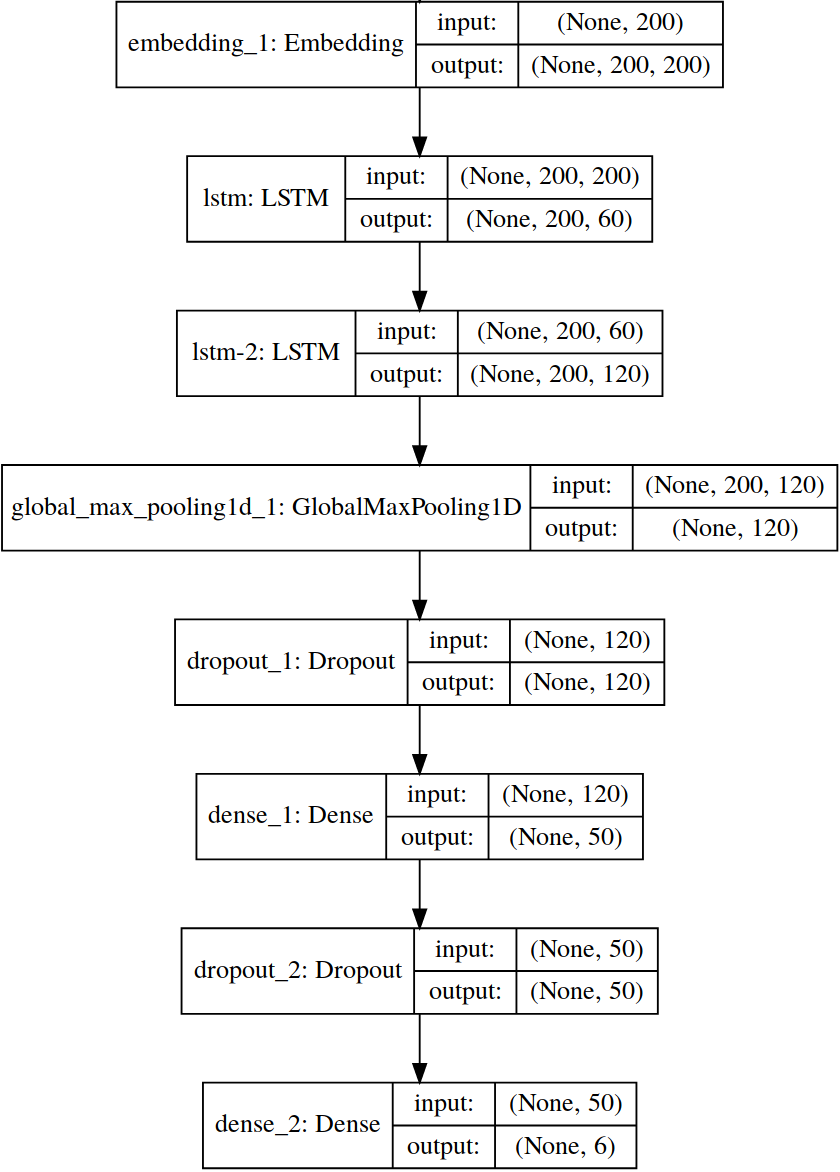
\includegraphics[height=10cm]{model-architecture.png}
		  \caption{RNN Model Architecture}
		  \label{fig:model-arch}
	  \end{figure}
  }
 }

\section{Results Analysis \textit{Gabriel Britain, Jonathan Innis}}{
  After completing all of our tuned hyperparameter runs, we extracted features
  from the Naive Bayes classifier, and viewed the words and phrases that
  contributed most to each classification. Selected results can be seen in
  Figure \ref{fig:features} on page \pageref{fig:features}.

  \begin{figure}
	  \textbf{toxic}
	  \begin{verbatim}
		yammer
		follarte
		fuckyourself
		crackhead
	\end{verbatim}
	  \textbf{severe toxic}
	  \begin{verbatim}
		stomes
		cartuchos
		ancestryearly
	\end{verbatim}
	  \textbf{obscene}
	  \begin{verbatim}
		achmed
		sexmist
		britch
		zigabo
	\end{verbatim}
	  \textbf{threat}
	  \begin{verbatim}
		m45terbate
		ma5terb8
		masterbat3
		zigabo
	\end{verbatim}
	  \textbf{insult}
	  \begin{verbatim}
		crackhead
		libtard
		suberbia
	\end{verbatim}
	  \textbf{identity hate}
	  \begin{verbatim}
		gomnna
		zigabo
		nebracka
	\end{verbatim}
	  \caption{Most Valuable Features}
	  \label{fig:features}
  \end{figure}

 }

\section{Conclusions \textit{Gabriel Britain, Jonathan Innis}}{
  After evaluating the results of each model, it can be concluded that the Naive
  Bayes classifier has the best performance; however, we believe that this is
  largely due to the significant imbalance of classes and the size of data. If
  more data was available, it makes sense that that the RNN would greatly
  benefit, and possibly surpass the Naive Bayes model. After this analysis, it
  can be concluded that the RNN with custom word embeddings would benefit the
  most from more data. Currently, the RNN built uses pre-trained word
  embeddings, but if provided more data, using custom word embeddings could
  provide better results.
 }



\pagebreak
\bibliography{bibliography}{}
\bibliographystyle{plain}
\end{document}